% ============================================================
% SLIDES DO SEMINÁRIO — Estimativa de Canal com Preâmbulo OFDM
% ============================================================
% Compilar com: pdflatex slides-seminario.tex
% Para ver notas do apresentador: \setbeameroption{show notes}
% ============================================================

\documentclass[aspectratio=169, 11pt]{beamer}

% --- Tema e cores ---
\usetheme{Madrid}
\usecolortheme{whale}
\setbeamertemplate{navigation symbols}{}
\setbeamertemplate{footline}[frame number]

% --- NOTAS DO APRESENTADOR ---
% Descomente a linha abaixo para VER as notas durante o estudo:
% \setbeameroption{show notes}
% Ou use show notes on second screen para apresentação com 2 telas:
% \setbeameroption{show notes on second screen=right}

% --- Pacotes ---
\usepackage[utf8]{inputenc}
\usepackage[T1]{fontenc}
\usepackage[brazil]{babel}
\usepackage{amsmath, amssymb}
\usepackage{graphicx}
\usepackage{booktabs}
\usepackage{tikz}
\usepackage{pgfplots}
\pgfplotsset{compat=1.18}
\usetikzlibrary{arrows.meta, positioning, calc, decorations.pathreplacing, patterns}
\usepackage{multimedia}

% --- Cores personalizadas ---
\definecolor{utfprblue}{RGB}{0, 83, 159}
\definecolor{utfprgold}{RGB}{255, 193, 7}
\definecolor{darkgreen}{RGB}{34, 139, 34}
\definecolor{highlight}{RGB}{230, 126, 34}

% --- Metadados ---
\title[Estimativa de Canal OFDM]{Estimativa de Canal Usando Preâmbulo OFDM:\\
Um Estudo Baseado em Simulações com a\\Biblioteca NVIDIA Sionna}
\subtitle{Tópicos em Redes sem Fio — Seminário Final}
\author[Maurice, Vinicius, Natalia]{
    Maurice Golin Soares dos Santos \and
    Vinicius Pereira Luz \and
    Natalia Mendes Goes
}
\institute[UTFPR]{
    Universidade Tecnológica Federal do Paraná (UTFPR)\\
    Ponta Grossa, PR\\[0.3cm]
    \textbf{Professor:} Saulo Jorge Beltrão de Queiroz
}
\date{Junho de 2026}

% ============================================================
\begin{document}

% ============================================================
% SLIDE 1: CAPA
% ============================================================
\begin{frame}[plain]
    \titlepage
\end{frame}

\note[itemize]{
    \item Cumprimentar o professor e a turma.
    \item Dizer: ``Nosso trabalho investiga como o receptor de um sistema 5G consegue descobrir o que aconteceu com o sinal no caminho entre a antena e o celular --- isso se chama estimativa de canal.''
    \item Mencionar que usamos uma ferramenta da NVIDIA chamada Sionna.
}

% ============================================================
% SLIDE 2: ROTEIRO
% ============================================================
\begin{frame}{O que vamos ver hoje?}
    \tableofcontents
    \vspace{0.3cm}
    \small\textit{Duração estimada: 15--20 minutos + perguntas}
\end{frame}

\note[itemize]{
    \item Explicar brevemente o roteiro: primeiro o ``porquê'', depois a teoria, depois o que fizemos, e finalmente os resultados.
}

% ============================================================
% SEÇÃO 1: MOTIVAÇÃO E OBJETIVOS
% ============================================================
\section{Motivação e Objetivos}

% ============================================================
% SLIDE 3: POR QUE ISSO IMPORTA?
% ============================================================
\begin{frame}{Por que a estimativa de canal importa?}

    \textbf{Imagine mandar uma carta pelo correio:}

    \pause
    \begin{itemize}
        \item Você escreve a carta (\textbf{sinal transmitido}) \pause
        \item O correio pode amassar, molhar ou perder trechos (\textbf{canal de propagação}) \pause
        \item O destinatário precisa \textbf{entender o que aconteceu com a carta} para reconstruir a mensagem original
    \end{itemize}

    \pause
    \vspace{0.5cm}
    \begin{block}{Em comunicações sem fio é a mesma ideia}
        O sinal de rádio sofre \textbf{reflexões}, \textbf{atenuações} e \textbf{ruído} no caminho até o receptor. Para decodificar os dados corretamente, o receptor precisa primeiro \textbf{descobrir o que o canal fez com o sinal}. Isso é a \textbf{estimativa de canal}.
    \end{block}

    \pause
    \vspace{0.3cm}
    \centering
    \textcolor{highlight}{\textbf{Se a estimativa for ruim → os dados chegam com erros!}}
\end{frame}

\note[itemize]{
    \item A analogia da carta é boa para começar. O canal é como o ``correio'' que pode danificar a mensagem.
    \item O ponto central: sem saber o que o canal fez, o receptor não consegue ``desfazer'' a distorção.
    \item Em sistemas reais (5G, Wi-Fi), a estimativa de canal acontece \textbf{milhares de vezes por segundo}.
    \item Dizer: ``Quanto melhor a estimativa, menos erros nos dados --- menos travamento no streaming, menos chamadas caindo.''
}

% ============================================================
% SLIDE 4: COMO O RECEPTOR DESCOBRE O CANAL?
% ============================================================
\begin{frame}{Como o receptor descobre o que o canal fez?}

    \textbf{A ideia é simples:} enviar algo \textbf{conhecido} pelo canal e ver como chegou.

    \pause
    \vspace{0.3cm}
    \begin{columns}[T]
        \begin{column}{0.55\textwidth}
            \begin{enumerate}
                \item O transmissor envia um \textbf{sinal de teste} conhecido (chamado \textbf{piloto}) \pause
                \item O receptor compara \textbf{o que recebeu} com \textbf{o que esperava} \pause
                \item A diferença revela \textbf{o efeito do canal}
            \end{enumerate}

            \pause
            \vspace{0.4cm}
            \textbf{Analogia:} é como enviar uma foto conhecida pelo fax. Se a foto chega borrada, você sabe exatamente quanto o fax borrou, e pode ``desborrar'' os documentos seguintes.
        \end{column}
        \begin{column}{0.42\textwidth}
            \begin{tikzpicture}[scale=0.8, every node/.style={font=\small}]
                % TX
                \node[draw, fill=blue!15, rounded corners, minimum width=2cm, minimum height=0.8cm] (tx) {TX};
                % RX
                \node[draw, fill=green!15, rounded corners, minimum width=2cm, minimum height=0.8cm, right=3cm of tx] (rx) {RX};
                % Canal
                \draw[-{Stealth}, thick, red!70, decorate, decoration={snake, amplitude=3pt, segment length=10pt}] (tx) -- node[above, black, font=\footnotesize] {Canal $H$} (rx);
                % Piloto
                \node[below=0.5cm of tx, font=\footnotesize, blue!70] {Envia: $X_p$ (conhecido)};
                \node[below=0.5cm of rx, font=\footnotesize, green!50!black] {Recebe: $Y_p = H \cdot X_p + W$};
                % Estimativa
                \node[below=1.5cm of rx, font=\footnotesize, red!70] {$\hat{H} = Y_p / X_p$};
                \draw[-{Stealth}, thick] ([yshift=-0.3cm]rx.south) -- ++(0, -0.7);
            \end{tikzpicture}
        \end{column}
    \end{columns}
\end{frame}

\note[itemize]{
    \item Esse slide explica a IDEIA CENTRAL de toda a estimativa de canal.
    \item Piloto = sinal de referência. É um ``sinal de teste'' que ambos (TX e RX) conhecem.
    \item $X_p$ é o que o TX envia, $Y_p$ é o que chega. A divisão $Y_p / X_p$ dá o efeito do canal $H$.
    \item A analogia do fax funciona bem: você envia uma imagem padrão, vê como chegou, e sabe como ``corrigir'' as próximas.
    \item Na prática, no 5G esses pilotos se chamam DMRS (Demodulation Reference Signals).
}

% ============================================================
% SLIDE 5: OBJETIVOS
% ============================================================
\begin{frame}{O que investigamos neste trabalho}
    \textbf{Pergunta central:}
    \begin{center}
        \textit{``Qual estimador de canal funciona melhor: o simples (LS) ou o avançado (LMMSE)?\\E quanto melhor?''}
    \end{center}

    \pause
    \vspace{0.4cm}
    \textbf{O que fizemos:}
    \begin{enumerate}
        \item Montamos um sistema OFDM completo (como no 5G) usando a biblioteca \textbf{Sionna} \pause
        \item Testamos com dois tipos de canal:
            \begin{itemize}
                \item \textbf{AWGN} — só ruído (caso ideal, fácil) \pause
                \item \textbf{CDL-C} — multipercurso + ruído (caso real, difícil)
            \end{itemize} \pause
        \item Medimos a \textbf{taxa de erro de bit} (BER) — quantos bits chegam errados \pause
        \item Comparamos os resultados com a teoria
    \end{enumerate}
\end{frame}

\note[itemize]{
    \item LS = Least Squares (mínimos quadrados). Mais simples. Divide e pronto.
    \item LMMSE = Linear Minimum Mean Square Error. Mais sofisticado. Usa informação estatística do canal.
    \item AWGN = canal perfeito + ruído. Como falar ao telefone numa sala silenciosa.
    \item CDL-C = canal com reflexões (multipercurso). Como falar ao telefone andando na rua.
    \item BER = se transmiti 1.000.000 bits e 100 chegaram errados, BER = $10^{-4}$.
}

% ============================================================
% SEÇÃO 2: FUNDAMENTAÇÃO TEÓRICA
% ============================================================
\section{Fundamentação Teórica}

% ============================================================
% SLIDE 6: O QUE É OFDM?
% ============================================================
\begin{frame}{O que é OFDM?}

    \textbf{OFDM = dividir a banda em muitas ``faixinhas'' (subportadoras)}

    \pause
    \vspace{0.3cm}
    \begin{columns}[T]
        \begin{column}{0.55\textwidth}
            \textbf{Analogia:} imagine uma rodovia com 64 faixas. Em vez de um caminhão gigante numa faixa só, você usa 64 carros pequenos, um em cada faixa. Se uma faixa tiver um buraco, só um carro é afetado!

            \pause
            \vspace{0.3cm}
            \textbf{Como funciona:}
            \begin{itemize}
                \item TX: dados $\xrightarrow{\text{IFFT}}$ sinal no tempo
                \item RX: sinal no tempo $\xrightarrow{\text{FFT}}$ dados
                \item \textbf{Prefixo cíclico (CP):} ``proteção'' contra ecos
            \end{itemize}

            \pause
            \vspace{0.3cm}
            \textbf{Usado em:} 4G LTE, \textbf{5G NR}, Wi-Fi
        \end{column}
        \begin{column}{0.42\textwidth}
            \begin{tikzpicture}[scale=0.65, every node/.style={font=\tiny}]
                % Subportadoras
                \foreach \i in {1,...,6} {
                    \draw[blue!\the\numexpr 20+\i*12\relax, thick, domain=0:4, samples=50]
                        plot (\x, {0.5*sin(deg(\x*\i*1.2))+ \i*0.8});
                }
                \node[right, font=\scriptsize] at (4.2, 5.6) {$f_6$};
                \node[right, font=\scriptsize] at (4.2, 4.8) {$f_5$};
                \node[right, font=\scriptsize] at (4.2, 4.0) {$f_4$};
                \node[right, font=\scriptsize] at (4.2, 3.2) {$f_3$};
                \node[right, font=\scriptsize] at (4.2, 2.4) {$f_2$};
                \node[right, font=\scriptsize] at (4.2, 1.6) {$f_1$};
                \node[below, font=\scriptsize] at (2, 0.5) {Cada ``onda'' é uma subportadora};
                \node[below, font=\scriptsize] at (2, 0) {carregando dados em paralelo};
            \end{tikzpicture}

            \vspace{0.3cm}
            \centering
            \begin{tikzpicture}[scale=0.6, every node/.style={font=\tiny}]
                \draw[fill=blue!15, draw=blue!60, thick] (0,0) rectangle (3.5,0.6);
                \node at (1.75, 0.3) {Símbolo OFDM ($N$)};
                \draw[fill=orange!25, draw=orange!70, thick] (-1.2,0) rectangle (0,0.6);
                \node at (-0.6, 0.3) {CP};
                \draw[-{Stealth}, dashed, red!70, thick] (2.8, -0.15) to[out=-20,in=-160] (-0.6, -0.15);
            \end{tikzpicture}

            \centering\scriptsize\vspace{0.1cm} CP = cópia do final
        \end{column}
    \end{columns}
\end{frame}

\note[itemize]{
    \item OFDM = Orthogonal Frequency-Division Multiplexing.
    \item A analogia da rodovia é essencial: se uma subportadora sofre desvanecimento profundo (``buraco''), as outras continuam funcionando.
    \item IFFT transforma dados (domínio da frequência) em sinal que pode ser transmitido (domínio do tempo).
    \item FFT no receptor faz o caminho inverso.
    \item O CP (prefixo cíclico) é uma cópia das últimas amostras colada no início. Ele ``absorve'' os ecos do multipercurso, evitando que um símbolo interfira no seguinte (ISI = Inter-Symbol Interference).
    \item Nosso sistema usa 76 subportadoras (64 efetivas), 14 símbolos OFDM por slot, espaçamento de 30 kHz --- configuração do 5G NR.
}

% ============================================================
% SLIDE 7: MODELO DO CANAL
% ============================================================
\begin{frame}{O que acontece com o sinal no canal?}

    \textbf{Modelo simplificado (no domínio da frequência):}
    \begin{equation*}
        \boxed{Y[k] = H[k] \cdot X[k] + W[k]}
    \end{equation*}

    \pause
    \vspace{0.2cm}
    \begin{center}
    \begin{tabular}{cl}
        $X[k]$ & = o que foi \textbf{enviado} na subportadora $k$ \\
        $H[k]$ & = o que o \textbf{canal fez} (atenuou? rotacionou a fase?) \\
        $W[k]$ & = \textbf{ruído} (sempre presente) \\
        $Y[k]$ & = o que foi \textbf{recebido}
    \end{tabular}
    \end{center}

    \pause
    \vspace{0.3cm}
    \begin{columns}[T]
        \begin{column}{0.48\textwidth}
            \textbf{Canal AWGN (fácil):}
            \begin{itemize}
                \item $H[k] = 1$ para todo $k$
                \item Sem distorção, só ruído
                \item Como falar ao telefone fixo
            \end{itemize}
        \end{column}
        \begin{column}{0.48\textwidth}
            \textbf{Canal CDL-C (realista):}
            \begin{itemize}
                \item $H[k]$ varia por subportadora
                \item Reflexões, ecos, atenuações
                \item Como falar no celular andando
            \end{itemize}
        \end{column}
    \end{columns}
\end{frame}

\note[itemize]{
    \item Essa equação é a mais importante de toda a apresentação.
    \item $Y = H \cdot X + W$ em palavras: ``o que recebo é o que enviei vezes o efeito do canal, mais ruído''.
    \item Se eu sei $X$ (piloto) e meço $Y$, posso calcular $H = Y/X$ (ignorando ruído).
    \item AWGN: $H=1$ significa que o canal não faz nada com o sinal, só adiciona ruído.
    \item CDL-C: o $H[k]$ varia --- em algumas frequências o canal atenua muito (deep fade), em outras passa bem. É o cenário real do 5G.
    \item CDL = Clustered Delay Line, modelo padronizado pelo 3GPP (organização que define o 5G).
}

% ============================================================
% SLIDE 8: GRADE DE RECURSOS — ONDE FICAM OS PILOTOS?
% ============================================================
\begin{frame}{Grade de recursos OFDM --- onde ficam os pilotos?}
    \begin{columns}[T]
        \begin{column}{0.45\textwidth}
            \begin{tikzpicture}[scale=0.42, every node/.style={font=\tiny}]
                \def\cols{14}
                \def\rows{10}
                \foreach \x in {0,...,\cols}{
                    \draw[gray!40] (\x, 0) -- (\x, \rows);
                }
                \foreach \y in {0,...,\rows}{
                    \draw[gray!40] (0, \y) -- (\cols, \y);
                }
                % Pilotos (símbolos 2 e 11)
                \foreach \y in {1,...,8}{
                    \fill[orange!50] (2, \y) rectangle (3, \y+1);
                    \fill[orange!50] (11, \y) rectangle (12, \y+1);
                }
                % Dados
                \foreach \x in {0,1,3,4,5,6,7,8,9,10,12,13}{
                    \foreach \y in {1,...,8}{
                        \fill[blue!15] (\x, \y) rectangle (\x+1, \y+1);
                    }
                }
                % Guarda
                \foreach \x in {0,...,13}{
                    \fill[gray!25] (\x, 9) rectangle (\x+1, 10);
                    \fill[gray!25] (\x, 0) rectangle (\x+1, 1);
                }
                % Labels
                \node[rotate=90, anchor=south] at (-0.8, 5) {\scriptsize Frequência (subportadoras)};
                \node[anchor=north] at (7, -0.3) {\scriptsize Tempo (símbolos OFDM)};
                % Legenda
                \fill[orange!50] (15, 8) rectangle (15.7, 8.7);
                \node[right] at (15.9, 8.35) {\scriptsize Pilotos};
                \fill[blue!15] (15, 6.5) rectangle (15.7, 7.2);
                \node[right] at (15.9, 6.85) {\scriptsize Dados};
                \fill[gray!25] (15, 5) rectangle (15.7, 5.7);
                \node[right] at (15.9, 5.35) {\scriptsize Guarda};
                % Indicadores
                \draw[{Stealth}-, thick, red!70] (2.5, 9.3) -- ++(0, 0.7) node[above, font=\scriptsize] {Piloto 1};
                \draw[{Stealth}-, thick, red!70] (11.5, 9.3) -- ++(0, 0.7) node[above, font=\scriptsize] {Piloto 2};
            \end{tikzpicture}
        \end{column}
        \begin{column}{0.52\textwidth}
            \textbf{O que é a grade de recursos?}
            \begin{itemize}
                \item Um ``tabuleiro'' onde cada célula carrega \textbf{um símbolo} \pause
                \item \textbf{Eixo horizontal:} tempo (14 símbolos OFDM) \pause
                \item \textbf{Eixo vertical:} frequência (64 subportadoras efetivas) \pause
                \item \textcolor{orange}{\textbf{Pilotos}} ficam nos símbolos 2 e 11 — ``sinais de teste'' \pause
                \item \textcolor{blue}{\textbf{Dados}} ficam no resto \pause
                \item \textcolor{gray}{\textbf{Guarda}} nas bordas (evita interferência)
            \end{itemize}

            \vspace{0.3cm}
            \textbf{O receptor:}
            \begin{enumerate}
                \item Usa os \textcolor{orange}{\textbf{pilotos}} para estimar $H[k]$
                \item \textbf{Interpola} para as posições de dados
                \item ``Desfaz'' o efeito do canal nos dados
            \end{enumerate}
        \end{column}
    \end{columns}
\end{frame}

\note[itemize]{
    \item A grade de recursos é como uma planilha do Excel: cada célula é um ``resource element'' (RE).
    \item Nosso sistema tem 14 colunas (símbolos OFDM no tempo) e 76 linhas (subportadoras), sendo 64 efetivas.
    \item Pilotos nos símbolos 2 e 11: o receptor estima o canal nesses dois momentos e interpola para o resto.
    \item Se o canal muda rápido (velocidade alta), precisa de mais pilotos. Se muda devagar, menos pilotos bastam.
    \item No 5G, esses pilotos se chamam DMRS (Demodulation Reference Signals).
    \item Nosso padrão de pilotos é ``Kronecker'' --- pilotos em todas as subportadoras efetivas nos símbolos escolhidos.
}

% ============================================================
% SLIDE 9: ESTIMADOR LS — O SIMPLES
% ============================================================
\begin{frame}{Estimador LS --- ``a divisão simples''}

    \textbf{Ideia:} se $Y = H \cdot X + W$, e eu conheço $X$ (piloto), então:
    \begin{equation*}
        \boxed{\hat{H}_{\text{LS}} = \frac{Y_{\text{piloto}}}{X_{\text{piloto}}}}
    \end{equation*}

    \pause
    \vspace{0.2cm}
    \textbf{Analogia:} é como medir a temperatura com um termômetro barato. Funciona, mas tem ``barulho'' na leitura.

    \pause
    \vspace{0.3cm}
    \begin{columns}[T]
        \begin{column}{0.48\textwidth}
            \textcolor{darkgreen}{\textbf{✓ Vantagens:}}
            \begin{itemize}
                \item Muito simples (só uma divisão!)
                \item Não precisa saber nada sobre o canal
                \item Complexidade $\mathcal{O}(N_p)$ — super rápido
            \end{itemize}
        \end{column}
        \begin{column}{0.48\textwidth}
            \textcolor{red}{\textbf{✗ Desvantagens:}}
            \begin{itemize}
                \item O ruído $W$ ``contamina'' a estimativa:
                    $$\hat{H} = H + \underbrace{\frac{W}{X_p}}_{\text{erro!}}$$
                \item Quanto mais ruído, pior a estimativa
                \item Ruim em SNR baixa
            \end{itemize}
        \end{column}
    \end{columns}
\end{frame}

\note[itemize]{
    \item LS = Least Squares = Mínimos Quadrados.
    \item A equação $\hat{H} = Y/X$ é intuitiva: ``divido o que recebi pelo que enviei''.
    \item O problema: a divisão também divide o ruído por $X$, amplificando-o.
    \item Se $X$ for grande (pilotos com alta potência), o erro é menor. Se $X$ for pequeno, o ruído amplificado explode.
    \item Na prática, o LS é usado como ``primeiro passo'' porque é muito barato computacionalmente.
    \item $N_p$ = número de pilotos. No nosso caso, são 64 pilotos por símbolo OFDM piloto.
    \item SNR = Signal-to-Noise Ratio. SNR alta = pouco ruído, SNR baixa = muito ruído.
}

% ============================================================
% SLIDE 10: ESTIMADOR LMMSE — O AVANÇADO
% ============================================================
\begin{frame}{Estimador LMMSE --- ``a média inteligente''}

    \textbf{Ideia:} pegar a estimativa LS (ruidosa) e \textbf{suavizar} usando o que sabemos sobre o canal.

    \pause
    \begin{equation*}
        \boxed{\hat{\mathbf{H}}_{\text{LMMSE}} = \underbrace{\mathbf{R}_{HH}}_{\text{correlação do canal}} \left(\mathbf{R}_{HH} + \underbrace{\frac{\sigma_w^2}{\sigma_x^2}}_{\text{nível de ruído}} \mathbf{I}\right)^{-1} \hat{\mathbf{H}}_{\text{LS}}}
    \end{equation*}

    \pause
    \vspace{0.2cm}
    \textbf{Analogia:} é como tirar uma foto com ruído e aplicar um filtro de ``suavização inteligente'' que sabe que pixels vizinhos devem ser parecidos.

    \pause
    \vspace{0.3cm}
    \centering
    \begin{tabular}{lcc}
        \toprule
        & \textbf{LS (simples)} & \textbf{LMMSE (avançado)} \\
        \midrule
        Complexidade & $\mathcal{O}(N_p)$ & $\mathcal{O}(N_p^3)$ \\
        Precisa saber sobre o canal? & Não & Sim ($\mathbf{R}_{HH}$, $\sigma_w^2$) \\
        Funciona bem com ruído? & \textcolor{red}{Não muito} & \textcolor{darkgreen}{\textbf{Sim}} \\
        Ganho típico & --- & \textbf{5 a 15 dB} \\
        \bottomrule
    \end{tabular}
\end{frame}

\note[itemize]{
    \item LMMSE = Linear Minimum Mean Square Error.
    \item $\mathbf{R}_{HH}$ é a matriz de autocorrelação: diz ``quanto as subportadoras vizinhas se parecem''. Subportadoras próximas têm $H[k]$ parecido $\to$ a matriz ``sabe'' disso e suaviza.
    \item O termo $\sigma_w^2 / \sigma_x^2$ é o inverso da SNR. Quanto mais ruído, mais o LMMSE suaviza.
    \item Em SNR alta: LMMSE $\approx$ LS (pouca suavização necessária).
    \item Em SNR baixa: LMMSE remove muito ruído que o LS não consegue.
    \item A desvantagem: precisa conhecer $\mathbf{R}_{HH}$ (estatísticas do canal) e é computacionalmente caro ($N_p^3$).
    \item Ganho de 5 a 15 dB: para ter o mesmo BER que o LS, o LMMSE precisa de 5 a 15 dB \textit{menos} de potência!
    \item Na nossa simulação, usamos LS para estimar o canal + LMMSE para equalizar (não LMMSE completo para estimativa).
}

% ============================================================
% SEÇÃO 3: MATERIAIS E MÉTODOS
% ============================================================
\section{Materiais e Métodos}

% ============================================================
% SLIDE 11: O QUE É O SIONNA?
% ============================================================
\begin{frame}{A ferramenta: NVIDIA Sionna}
    \begin{columns}[T]
        \begin{column}{0.55\textwidth}
            \textbf{O que é:} biblioteca Python \textit{open-source} da NVIDIA para simular sistemas de comunicação sem fio.

            \pause
            \vspace{0.3cm}
            \textbf{Por que usamos:}
            \begin{itemize}
                \item Tem \textbf{todos os blocos prontos}: codificador, modulador, canal, estimador...
                \item Segue os padrões \textbf{3GPP do 5G NR}
                \item Roda em \textbf{GPU} (rápido) ou CPU
                \item É \textbf{gratuito} e reproduzível
            \end{itemize}

            \pause
            \vspace{0.3cm}
            \textbf{Nosso ambiente:}\\
            \small Python 3.13 + Sionna 2.0.1 + PyTorch\\
            Execução em CPU (sem GPU)
        \end{column}
        \begin{column}{0.42\textwidth}
            \centering\textbf{Cadeia de processamento:}
            \vspace{0.2cm}

            \begin{tikzpicture}[
                block/.style={rectangle, draw, fill=#1, minimum height=0.4cm, minimum width=1.7cm, align=center, font=\tiny, rounded corners=2pt, thick},
                arrow/.style={-{Stealth}, thick},
                node distance=0.18cm
            ]
                \node[block=blue!15] (bs) {Gera bits};
                \node[block=blue!15, below=of bs] (enc) {Codifica (LDPC)};
                \node[block=blue!15, below=of enc] (map) {Modula (16-QAM)};
                \node[block=blue!15, below=of map] (rgm) {Insere pilotos};
                \node[block=blue!15, below=of rgm] (omod) {OFDM (IFFT+CP)};
                \node[block=red!15, below=0.3cm of omod] (ch) {\textbf{Canal}};
                \node[block=green!15, below=0.3cm of ch] (odem) {OFDM (FFT)};
                \node[block=yellow!25, below=of odem] (est) {\textbf{Estima canal (LS)}};
                \node[block=green!15, below=of est] (eql) {Equaliza (LMMSE)};
                \node[block=green!15, below=of eql] (dem) {Demodula};
                \node[block=green!15, below=of dem] (dec) {Decodifica (LDPC)};

                \draw[arrow] (bs) -- (enc);
                \draw[arrow] (enc) -- (map);
                \draw[arrow] (map) -- (rgm);
                \draw[arrow] (rgm) -- (omod);
                \draw[arrow] (omod) -- (ch);
                \draw[arrow] (ch) -- (odem);
                \draw[arrow] (odem) -- (est);
                \draw[arrow] (est) -- (eql);
                \draw[arrow] (eql) -- (dem);
                \draw[arrow] (dem) -- (dec);
            \end{tikzpicture}
        \end{column}
    \end{columns}
\end{frame}

\note[itemize]{
    \item O Sionna foi criado pelo time de pesquisa da NVIDIA em 2022 (paper no arXiv).
    \item Cada ``caixinha'' no diagrama é um módulo do Sionna. É como montar Lego: você encaixa os blocos.
    \item LDPC = Low-Density Parity-Check. É o código de correção de erros usado no 5G. Muito poderoso!
    \item 16-QAM = cada símbolo carrega 4 bits (16 pontos na constelação).
    \item O fluxo é: bits $\to$ codifica $\to$ modula $\to$ coloca na grade OFDM $\to$ transmite $\to$ canal distorce $\to$ receptor desfaz tudo na ordem inversa.
    \item Nós usamos: estimativa LS + equalização LMMSE. Ou seja, a estimativa é simples (LS), mas a equalização é sofisticada (LMMSE).
}

% ============================================================
% SLIDE 12: PARÂMETROS
% ============================================================
\begin{frame}{Configuração da simulação}
    \begin{columns}[T]
        \begin{column}{0.48\textwidth}
            \textbf{Sistema OFDM:}
            \small
            \begin{tabular}{lr}
                \toprule
                \textbf{Parâmetro} & \textbf{Valor} \\
                \midrule
                Subportadoras (FFT) & 76 (64 úteis) \\
                Símbolos OFDM/slot & 14 \\
                Espaçamento & 30 kHz \\
                Prefixo cíclico & 6 amostras \\
                Modulação & 16-QAM \\
                Código & LDPC $R=1/2$ \\
                Pilotos & Kronecker \\
                Batch size & 128 \\
                \bottomrule
            \end{tabular}
        \end{column}
        \begin{column}{0.48\textwidth}
            \textbf{Canal CDL-C (3GPP):}
            \small
            \begin{tabular}{lr}
                \toprule
                \textbf{Parâmetro} & \textbf{Valor} \\
                \midrule
                Perfil & CDL-C (NLOS) \\
                Delay spread & 100 ns \\
                Portadora & 3.5 GHz \\
                Velocidade & 3 m/s \\
                Antenas & SISO (1$\times$1) \\
                \bottomrule
            \end{tabular}

            \vspace{0.5cm}
            \textbf{Métrica:} BER (Bit Error Rate)
            $$\text{BER} = \frac{\text{bits errados}}{\text{total de bits}}$$

            \small 196.608 bits testados por ponto
        \end{column}
    \end{columns}
\end{frame}

\note[itemize]{
    \item 76 subportadoras = FFT de tamanho 76. Dessas, 64 são efetivas (as outras são guarda e DC nula).
    \item 14 símbolos OFDM por slot = padrão do 5G NR.
    \item 30 kHz de espaçamento entre subportadoras = banda n78 (3.5 GHz), frequência típica do 5G no Brasil.
    \item LDPC com taxa $R = 1/2$: metade dos bits transmitidos são redundância para correção de erros. Isso permite recuperar dados mesmo com bastante ruído.
    \item Batch size = 128: transmitimos 128 ``pacotes'' por ponto de SNR. Cada pacote tem 1536 bits de informação. Total = 128 $\times$ 1536 = 196.608 bits.
    \item CDL-C: cenário urbano sem linha de visada, 24 clusters de reflexão, delay spread de 100 ns.
    \item SISO = Single-Input Single-Output (uma antena TX, uma antena RX). É o caso mais simples.
}

% ============================================================
% SEÇÃO 4: RESULTADOS
% ============================================================
\section{Resultados}

% ============================================================
% SLIDE 13: GRADE DE RECURSOS (GERADA)
% ============================================================
\begin{frame}{Resultado: grade de recursos gerada pelo Sionna}
    \centering
    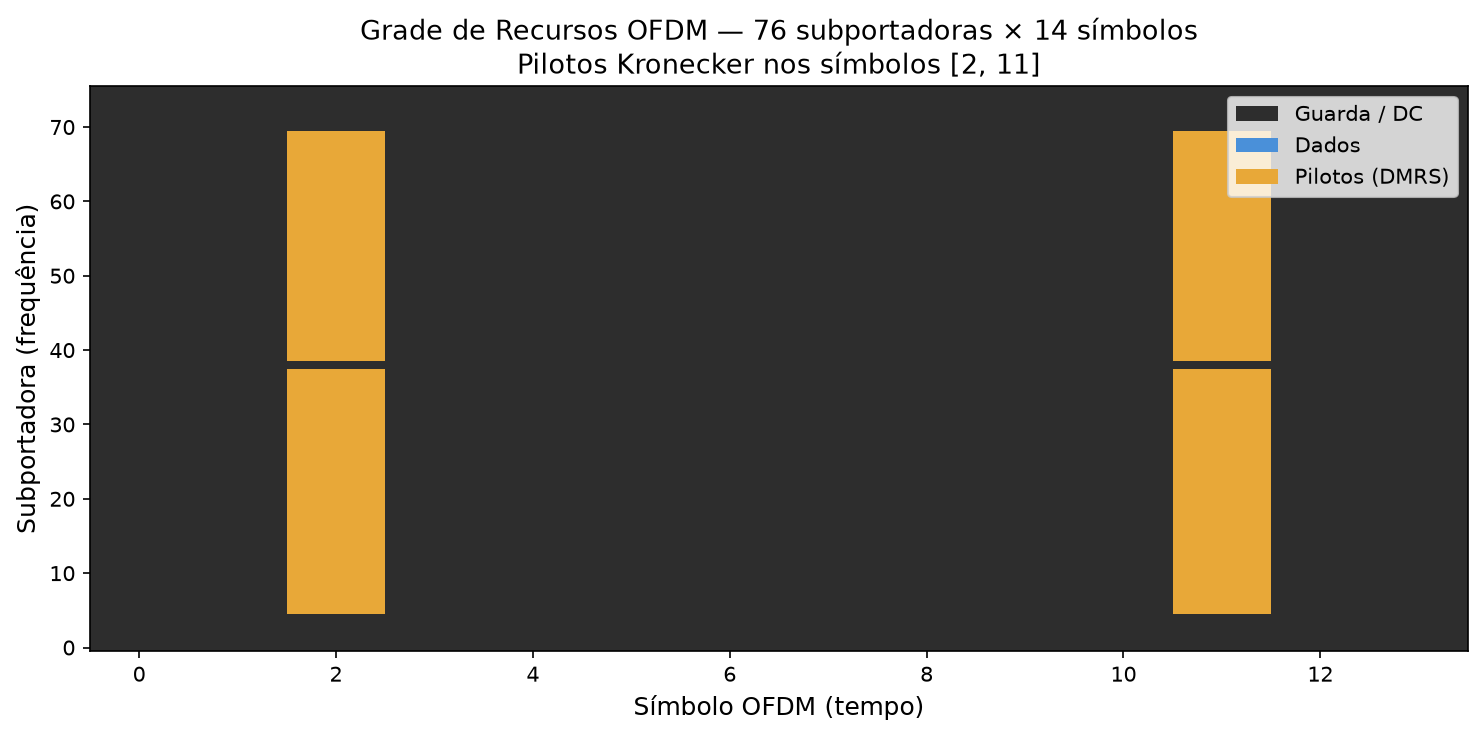
\includegraphics[width=0.72\textwidth]{figs/grade_recursos_ofdm.png}

    \vspace{0.2cm}
    \small Os pilotos Kronecker (laranja) ocupam os símbolos OFDM 2 e 11.\\
    Dados do usuário (azul) preenchem as demais posições.\\
    Guarda e DC nula (escuro) nas bordas.
\end{frame}

\note[itemize]{
    \item Esse gráfico foi gerado automaticamente pelo nosso script Python.
    \item Observe que os pilotos (laranja) cobrem TODAS as subportadoras efetivas nos símbolos 2 e 11.
    \item Isso permite ao receptor estimar o canal em todas as frequências nesses dois instantes de tempo.
    \item Entre os pilotos (símbolos 3 a 10), o receptor interpola a estimativa.
    \item As faixas escuras no topo e no fundo são as subportadoras de guarda --- proteção contra interferência com canais adjacentes.
}

% ============================================================
% SLIDE 14: BER x Eb/N0 — O RESULTADO PRINCIPAL
% ============================================================
\begin{frame}{Resultado principal: curvas de BER}
    \begin{columns}[T]
        \begin{column}{0.56\textwidth}
            \centering
            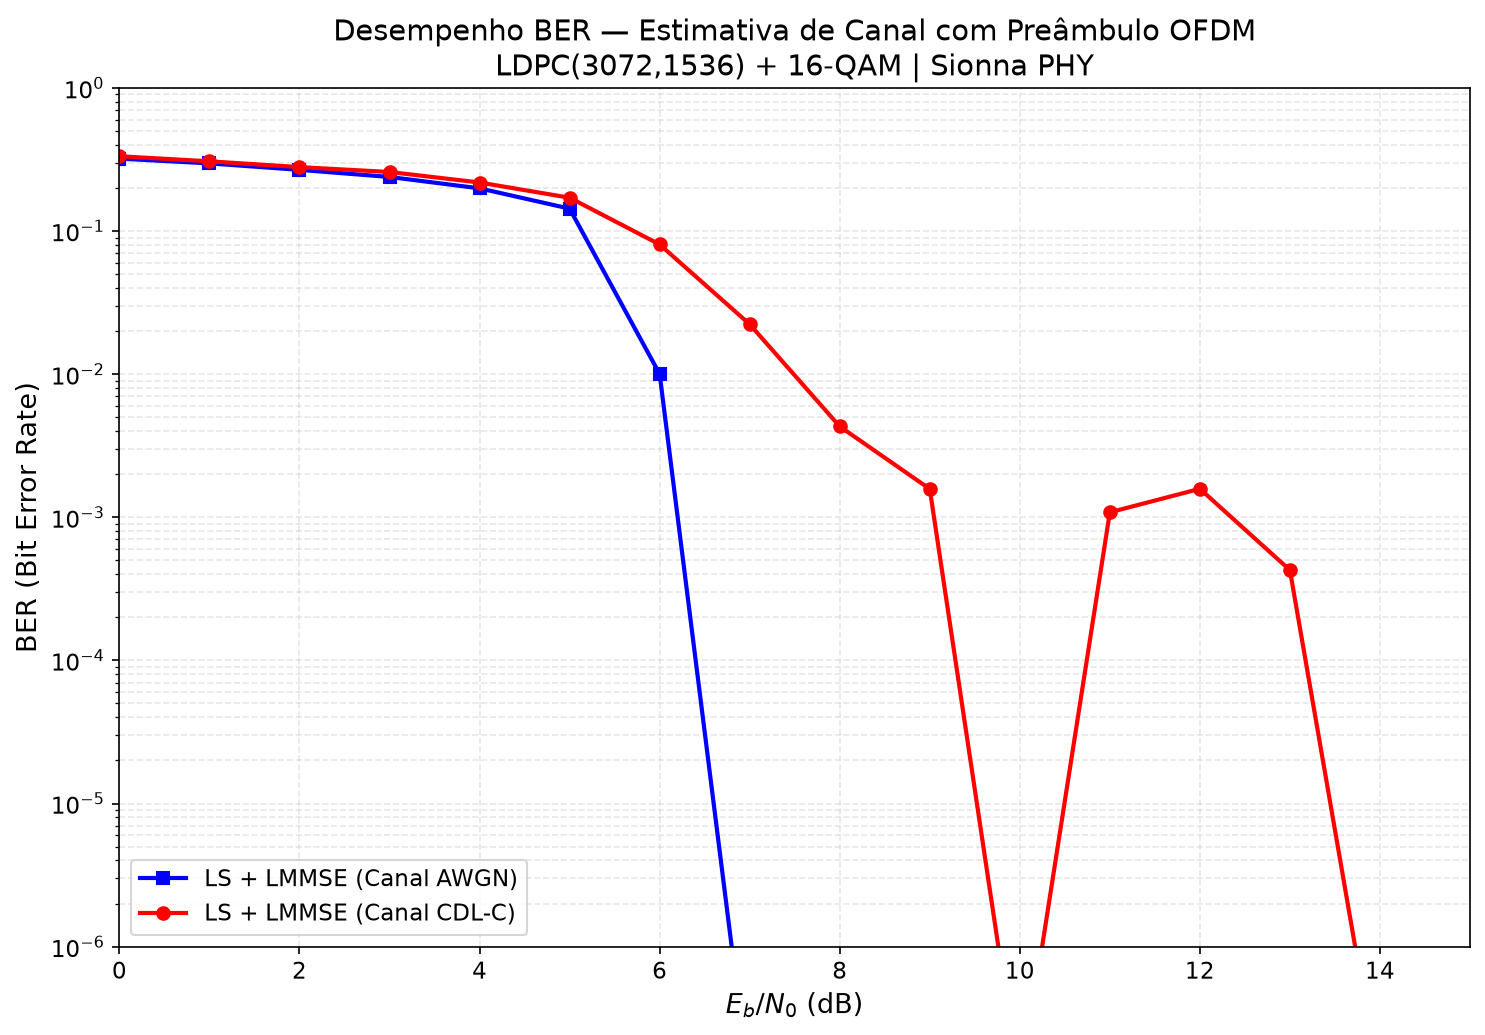
\includegraphics[width=\textwidth]{figs/ber_awgn_vs_cdl.png}
        \end{column}
        \begin{column}{0.42\textwidth}
            \pause
            \textbf{O que o gráfico mostra:}

            \vspace{0.2cm}
            \textbf{\textcolor{blue}{Azul (AWGN):}}
            \begin{itemize}\small
                \item BER cai rapidamente
                \item \textbf{BER = 0} a partir de 7 dB
                \item ``Efeito cascata'' do LDPC
            \end{itemize}

            \pause
            \vspace{0.2cm}
            \textbf{\textcolor{red}{Vermelho (CDL-C):}}
            \begin{itemize}\small
                \item BER cai mais devagar
                \item BER $\leq 10^{-3}$ em $\sim$10 dB
                \item Flutuações (canal aleatório)
            \end{itemize}

            \pause
            \vspace{0.3cm}
            \begin{block}{Penalidade}
                CDL-C precisa de \textbf{$\approx$ 3 dB a mais} que o AWGN para o mesmo BER
            \end{block}
        \end{column}
    \end{columns}
\end{frame}

\note[itemize]{
    \item ESTE é o gráfico mais importante do trabalho. Curva BER $\times$ Eb/N0.
    \item Eixo X: Eb/N0 em dB = ``qualidade do sinal''. Quanto maior, menos ruído relativo.
    \item Eixo Y: BER em escala log. $10^{-3}$ = 1 erro a cada 1000 bits.
    \item AWGN (azul): a BER despenca entre 6 e 7 dB. Isso é o ``waterfall'' do LDPC --- o código LDPC tem um limiar: abaixo dele, não funciona; acima, decodifica quase perfeitamente.
    \item CDL-C (vermelho): a curva desce mais devagar porque o canal com multipercurso dificulta a estimativa. O estimador LS erra mais em subportadoras com deep fade.
    \item Penalidade de 3 dB: significa que no CDL-C precisamos do \textit{dobro} de potência (3 dB = 2x) para o mesmo BER.
    \item Isso é consistente com a literatura (van de Beek, 1995 reporta 3--5 dB).
    \item As flutuações no CDL-C em 10--12 dB são porque cada execução gera um canal diferente (aleatório). Com batch maior, a curva ficaria mais suave.
}

% ============================================================
% SLIDE 15: TABELA DE RESULTADOS
% ============================================================
\begin{frame}{Resultados numéricos}
    \centering
    \small
    \begin{tabular}{rcc}
        \toprule
        $E_b/N_0$ (dB) & BER (AWGN) & BER (CDL-C) \\
        \midrule
        0  & $3{,}21 \times 10^{-1}$ & $3{,}33 \times 10^{-1}$ \\
        2  & $2{,}68 \times 10^{-1}$ & $2{,}80 \times 10^{-1}$ \\
        4  & $1{,}99 \times 10^{-1}$ & $2{,}18 \times 10^{-1}$ \\
        \rowcolor{blue!8}
        6  & $1{,}00 \times 10^{-2}$ & $8{,}06 \times 10^{-2}$ \\
        \rowcolor{blue!15}
        7  & \textbf{0} & $2{,}23 \times 10^{-2}$ \\
        8  & 0 & $4{,}31 \times 10^{-3}$ \\
        \rowcolor{red!8}
        10 & 0 & \textbf{0} \\
        14--15 & 0 & 0 \\
        \bottomrule
    \end{tabular}

    \pause
    \vspace{0.4cm}
    \begin{columns}[T]
        \begin{column}{0.48\textwidth}
            \centering
            \textcolor{blue}{\textbf{AWGN:}} BER = 0 em \textbf{7 dB}\\
            \small(limiar do LDPC)
        \end{column}
        \begin{column}{0.48\textwidth}
            \centering
            \textcolor{red}{\textbf{CDL-C:}} BER $\approx$ 0 em \textbf{10 dB}\\
            \small(3 dB de penalidade)
        \end{column}
    \end{columns}
\end{frame}

\note[itemize]{
    \item Essa tabela complementa o gráfico com os valores exatos.
    \item Destaque para a transição AWGN: de $10^{-2}$ em 6 dB para 0 em 7 dB. Isso é o waterfall!
    \item No CDL-C, a BER de $10^{-3}$ é alcançada em 9--10 dB.
    \item A não-monotonicidade no CDL-C (BER volta a subir em 11-12 dB) é porque o canal é ALEATÓRIO --- em algumas realizações, por azar, há deep fades severos nas posições dos pilotos.
    \item Com batch size maior (ex: 4096 em vez de 128), a média ficaria mais suave.
    \item BER = 0 não significa ``perfeito para sempre'' --- significa que nos 196.608 bits testados, nenhum errou.
}

% ============================================================
% SLIDE 16: RESPOSTA DO CANAL
% ============================================================
\begin{frame}{Como a estimativa LS se compara ao canal real?}
    \begin{columns}[T]
        \begin{column}{0.58\textwidth}
            \centering
            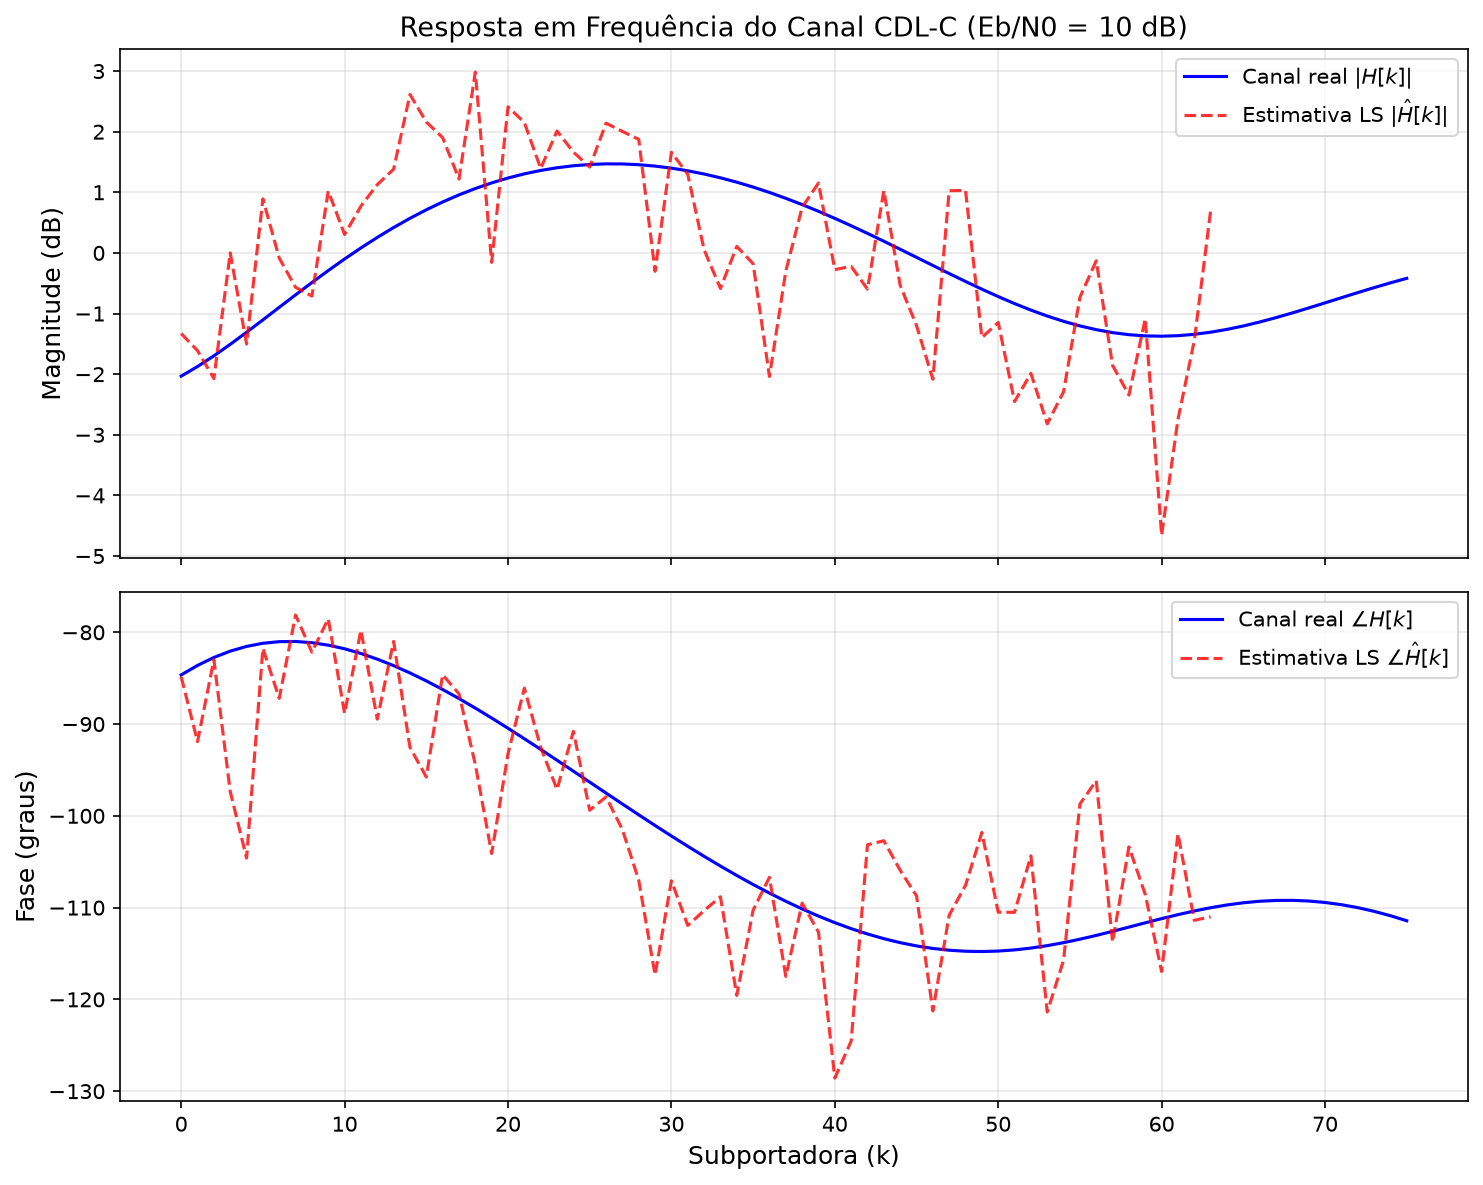
\includegraphics[width=\textwidth]{figs/canal_frequencia_real_vs_estimado.png}
        \end{column}
        \begin{column}{0.4\textwidth}
            \textbf{O que vemos:}
            \begin{itemize}\small
                \item \textcolor{blue}{\textbf{Azul:}} canal real $H[k]$\\ (o que realmente aconteceu) \pause
                \item \textcolor{red}{\textbf{Vermelho:}} estimativa LS $\hat{H}[k]$\\ (o que o receptor calculou) \pause
                \item O LS \textbf{acompanha a tendência}... \pause
                \item ...mas com \textbf{oscilações de $\pm$3 dB}
            \end{itemize}

            \pause
            \vspace{0.3cm}
            \textbf{Conclusão:}\\
            O LS funciona, mas é ``ruidoso''. O LMMSE suavizaria essas oscilações.
        \end{column}
    \end{columns}
\end{frame}

\note[itemize]{
    \item Esse gráfico mostra a ``fotografia'' do canal em um instante ($Eb/N0 = 10$ dB).
    \item Gráfico de cima: magnitude $|H[k]|$ em dB. O canal real (azul) varia suavemente. O LS (vermelho tracejado) oscila em volta.
    \item Gráfico de baixo: fase $\angle H[k]$. A fase real é quase linear (atraso de grupo constante). O LS tem mais desvios.
    \item Os desvios são maiores nas subportadoras onde $|H[k]|$ é pequeno (deep fade) --- a SNR local é menor ali.
    \item Se usássemos LMMSE completo para estimativa (e não só para equalização), as curvas vermelhas seriam muito mais suaves.
    \item Esse é um dos argumentos centrais do artigo: o LS é bom o suficiente, mas o LMMSE seria melhor.
}

% ============================================================
% SLIDE 17: CONSTELAÇÃO
% ============================================================
\begin{frame}{Efeito no diagrama de constelação}
    \centering
    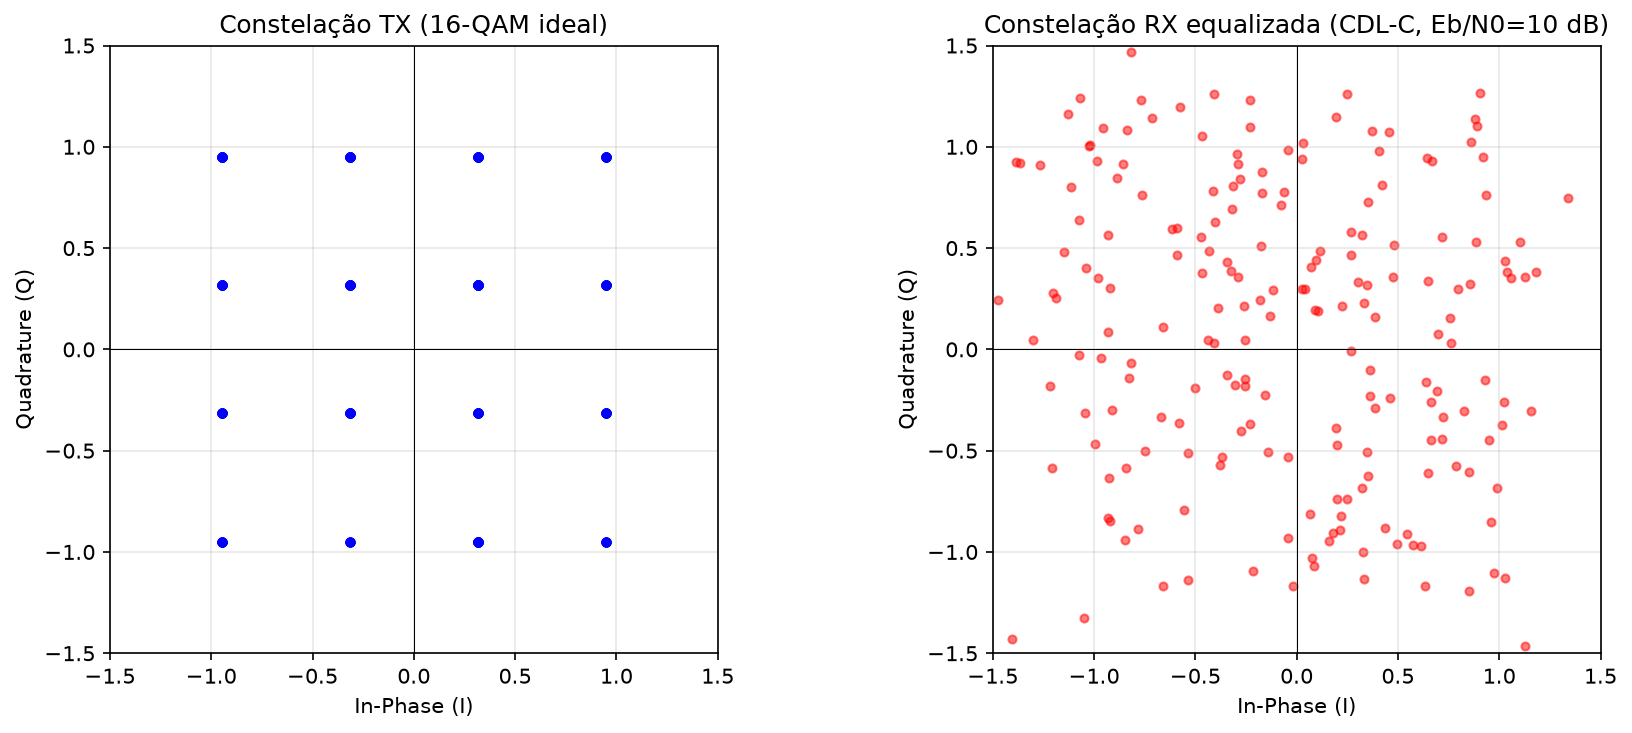
\includegraphics[width=0.75\textwidth]{figs/constelacao_tx_vs_rx.png}

    \pause
    \vspace{0.2cm}
    \begin{columns}[T]
        \begin{column}{0.48\textwidth}
            \centering
            \textbf{Esquerda: TX (ideal)}\\
            \small 16 pontos perfeitos na grade $4 \times 4$
        \end{column}
        \begin{column}{0.48\textwidth}
            \centering
            \textbf{Direita: RX equalizado}\\
            \small Pontos ``espalhados'' pelo ruído residual
        \end{column}
    \end{columns}

    \vspace{0.2cm}
    \small\textit{Quanto mais espalhado, mais difícil decidir qual ponto era. Pontos internos (menor energia) erram mais.}
\end{frame}

\note[itemize]{
    \item 16-QAM: 16 pontos no plano complexo (I vs Q). Cada ponto carrega 4 bits.
    \item Na transmissão, os pontos estão perfeitos (esquerda).
    \item Após o canal CDL-C + estimativa LS + equalização LMMSE, os pontos se ``espalham'' (direita).
    \item Os pontos mais ao centro (menor amplitude) se espalham mais e podem ``invadir'' a região do vizinho --- gerando erro.
    \item Os pontos nos cantos (maior amplitude) ficam mais concentrados --- mais resistentes ao ruído.
    \item A dispersão reflete o ruído que a equalização não conseguiu remover completamente.
    \item Quanto melhor a estimativa de canal, menor a dispersão e menor a BER.
}

% ============================================================
% SEÇÃO 5: DISCUSSÃO
% ============================================================
\section{Discussão e Conclusão}

% ============================================================
% SLIDE 18: ANÁLISE — O QUE APRENDEMOS?
% ============================================================
\begin{frame}{O que aprendemos com os resultados?}

    \begin{enumerate}
        \item \textbf{O estimador LS funciona}, mas paga uma penalidade em canais reais \pause

        \vspace{0.2cm}
        \item \textbf{Penalidade de $\approx$ 3 dB} do CDL-C vs AWGN\\
            \small $\to$ Precisa do dobro de potência para o mesmo BER\\
            $\to$ Consistente com a literatura (van de Beek, 1995) \pause

        \vspace{0.2cm}
        \item \normalsize \textbf{O código LDPC tem efeito ``cascata''}\\
            \small $\to$ Abaixo do limiar: muitos erros. Acima: quase zero erros.\\
            $\to$ No AWGN, o limiar ficou entre 6--7 dB \pause

        \vspace{0.2cm}
        \item \normalsize \textbf{O LMMSE completo melhoraria em 2--5 dB}\\
            \small $\to$ Nós usamos LS para estimar + LMMSE para equalizar\\
            $\to$ Usar LMMSE para estimar também reduziria o ``ruído'' da Fig.~5 \pause

        \vspace{0.2cm}
        \item \normalsize \textbf{O Sionna é uma ferramenta poderosa e acessível}\\
            \small $\to$ Módulos prontos conforme padrões 3GPP\\
            $\to$ Gratuito, open-source, documentado
    \end{enumerate}
\end{frame}

\note[itemize]{
    \item Este slide resume as conclusões do trabalho de forma didática.
    \item Ponto 1: O LS é o estimador mais simples possível, e mesmo assim funciona razoavelmente.
    \item Ponto 2: 3 dB de penalidade = precisa de 2x mais potência. Em termos práticos, isso significa torre com mais potência ou menor distância ao celular.
    \item Ponto 3: LDPC é um código ``tudo ou nada''. Isso é bom: quando funciona, funciona muito bem.
    \item Ponto 4: Se tivéssemos implementado o LMMSE completo (estimativa + equalização), o CDL-C teria desempenho mais próximo do AWGN.
    \item Ponto 5: O Sionna permite fazer em poucas centenas de linhas de Python o que antes exigia simuladores proprietários caros (como MATLAB).
    \item Se perguntarem ``por que não implementaram o LMMSE completo?'': dizer que fica como trabalho futuro e que a comparação LS vs canal ideal já demonstra o conceito.
}

% ============================================================
% SLIDE 19: CONCLUSÃO
% ============================================================
\begin{frame}{Conclusão}
    \textbf{O que fizemos:}
    \begin{itemize}
        \item Implementamos um sistema OFDM completo conforme 5G NR
        \item Avaliamos estimativa de canal LS em cenários AWGN e CDL-C
        \item Quantificamos a penalidade de SNR ($\approx$ 3 dB)
        \item Validamos resultados com a literatura
    \end{itemize}

    \pause
    \vspace{0.5cm}
    \textbf{Trabalhos futuros:}
    \begin{itemize}
        \item Implementar estimador LMMSE completo (não só equalização)
        \item Testar com QPSK e 64-QAM
        \item Extensão para \textbf{MIMO} (múltiplas antenas)
        \item Receptores baseados em \textbf{redes neurais} (\textit{neural receivers})
    \end{itemize}
\end{frame}

\note[itemize]{
    \item Resumir de forma confiante: ``Mostramos que o LS funciona, mas com limitações. O LMMSE melhoraria o desempenho, o que fica como trabalho futuro.''
    \item MIMO = Multiple-Input Multiple-Output. Múltiplas antenas no TX e RX. É o que o 5G usa na prática (massive MIMO com 64+ antenas).
    \item Neural receivers: usar redes neurais para substituir os blocos clássicos (estimador + equalizador) --- o Sionna já tem tutorial sobre isso!
    \item Se houver tempo, mencionar que o Sionna permite treinar esses receptores neurais porque toda a cadeia é diferenciável (backpropagation).
}

% ============================================================
% SLIDE 20: CÓDIGO-FONTE
% ============================================================
\begin{frame}[fragile]{Código-fonte}
    \textbf{Repositório:} \url{https://github.com/mauricegss/sionna}

    \vspace{0.3cm}
    \begin{columns}[T]
        \begin{column}{0.48\textwidth}
            \textbf{Estrutura:}
\begin{verbatim}
sionna/
├── article/
│   ├── artigo-final.tex
│   ├── slides-seminario.tex
│   └── figs/  (gráficos)
├── main/
│   ├── ofdm_channel_estimation.py
│   └── output/  (resultados)
├── experiments/
│   └── hello-world.py
└── README.md
\end{verbatim}
        \end{column}
        \begin{column}{0.48\textwidth}
            \textbf{Para reproduzir:}
\begin{verbatim}
# 1. Clonar
git clone <url>
cd sionna

# 2. Instalar
pip install sionna

# 3. Executar
python main/ofdm_channel_estimation.py
\end{verbatim}

            \vspace{0.3cm}
            \small\textbf{Tempo de execução:}\\
            $\sim$2--5 min (CPU)\\
            $\sim$30 seg (GPU)
        \end{column}
    \end{columns}
\end{frame}

\note[itemize]{
    \item Mostrar que o código está disponível e é reproduzível.
    \item O script principal é \texttt{ofdm\_channel\_estimation.py} com $\sim$750 linhas.
    \item Ele gera automaticamente os 4 gráficos + relatório TXT + CSV.
    \item O \texttt{hello-world.py} é o primeiro experimento (mais simples, sem OFDM).
    \item Se alguém quiser reproduzir: basta `pip install sionna` e rodar.
}

% ============================================================
% SLIDE 21: REFERÊNCIAS
% ============================================================
\begin{frame}{Referências principais}
    \small
    \begin{enumerate}
        \item Hoydis, J. et al. ``Sionna: An Open-Source Library for Next-Generation Physical Layer Research.'' \textit{arXiv:2203.11854}, 2022.
        \item Proakis, J. G.; Salehi, M. \textit{Digital Communications}. 5ª ed. McGraw-Hill, 2008.
        \item Goldsmith, A. \textit{Wireless Communications}. Cambridge Univ. Press, 2005.
        \item van de Beek, J.-J. et al. ``On channel estimation in OFDM systems.'' \textit{Proc. IEEE VTC}, 1995.
        \item Edfors, O. et al. ``OFDM channel estimation by singular value decomposition.'' \textit{IEEE Trans. Commun.}, 1998.
        \item 3GPP TS 38.211 / TR 38.901.
        \item Documentação NVIDIA Sionna: \url{https://nvlabs.github.io/sionna/}
    \end{enumerate}
\end{frame}

% ============================================================
% SLIDE 22: OBRIGADO
% ============================================================
\begin{frame}[plain]
    \centering
    \vfill
    {\Huge\textbf{Obrigado!}}

    \vspace{1cm}
    {\large Perguntas?}

    \vspace{1.5cm}
    \small
    Maurice Golin Soares dos Santos\\
    Vinicius Pereira Luz\\
    Natalia Mendes Goes\\[0.5cm]
    \textit{Tópicos em Redes sem Fio — UTFPR Ponta Grossa}\\
    Junho de 2026
    \vfill
\end{frame}

\note[itemize]{
    \item Agradecer ao professor e à turma.
    \item Abrir para perguntas.
    \item Possíveis perguntas e respostas preparadas:
    \item \textbf{``Por que não implementaram LMMSE completo?''} $\to$ ``Ficou como trabalho futuro. O foco foi demonstrar o sistema completo e quantificar a penalidade do canal realista.''
    \item \textbf{``Por que o CDL-C e não outro?''} $\to$ ``CDL-C representa cenário urbano NLOS com espalhamento moderado, que é o cenário mais comum do 5G.''
    \item \textbf{``O que é BER aceitável?''} $\to$ ``Em comunicações, $10^{-3}$ a $10^{-5}$ é típico. O 5G visa BER $\leq 10^{-5}$ após decodificação.''
    \item \textbf{``Funciona sem GPU?''} $\to$ ``Sim! Rodamos tudo em CPU. GPU só acelera.''
}

\end{document}
